\subsection{Simulation}

\begin{frame}{Simulation}{LOS Coverage Map}
  \begin{block}{Parameters taken into account for map simulation:}

	  \begin{itemize}
	  	\item Terrain elevation
	  	\item Curvature of the Earth
	  	\item Altitude of UA and GS
	  \end{itemize}

	  \begin{figure}
        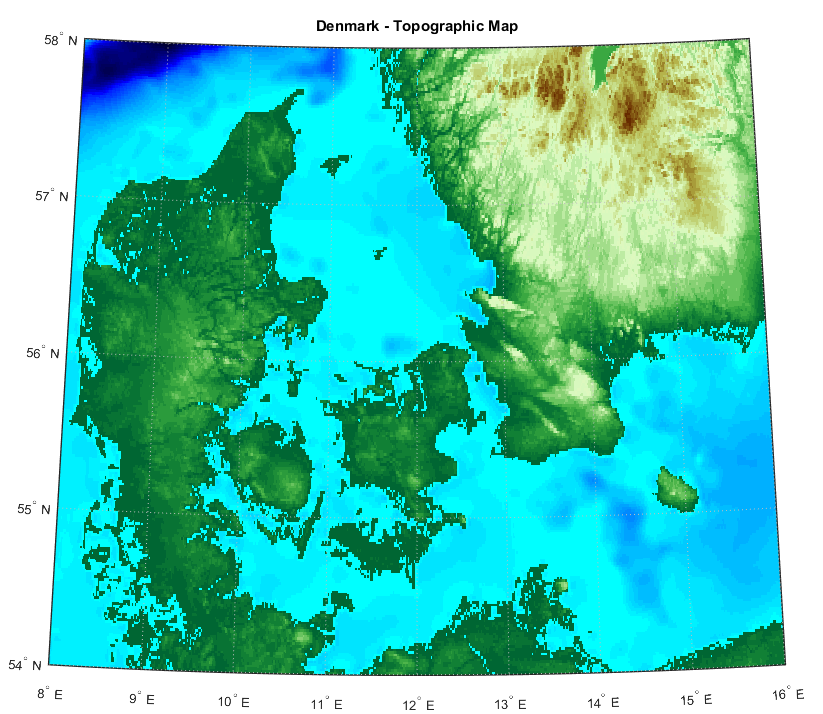
\includegraphics[scale=0.26]{../report/figures/dk_map.png}
      \end{figure}
  
  \end{block}
\end{frame}

\begin{frame}{Simulation}{LOS Coverage Map}
  \begin{block}{Working Principle}
	  \begin{itemize}
	  	\item Import topography map
	  	\item Input GS and UA altitude
	  	\item Choose GS and UA locations on map to plot LOS distance
	  	\item Choose GS location on map to plot LOS coverage map
	  \end{itemize}
  \end{block}
\end{frame}

\begin{frame}{Simulation}{LOS between UA and GS} 
  	\begin{figure}
        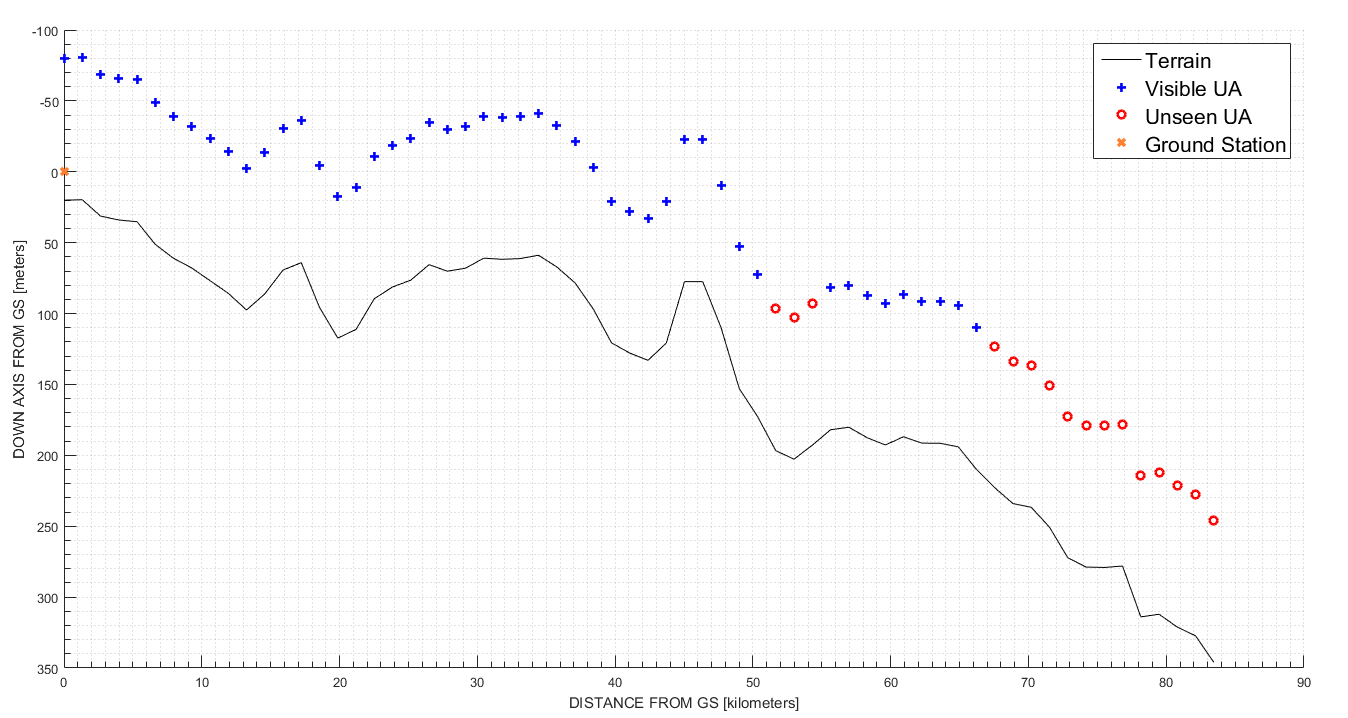
\includegraphics[scale=0.29]{../report/figures/los_2points.png}
    \end{figure}
\end{frame}

\begin{frame}{Simulation}{LOS Coverage Map} 
  	\begin{figure}
        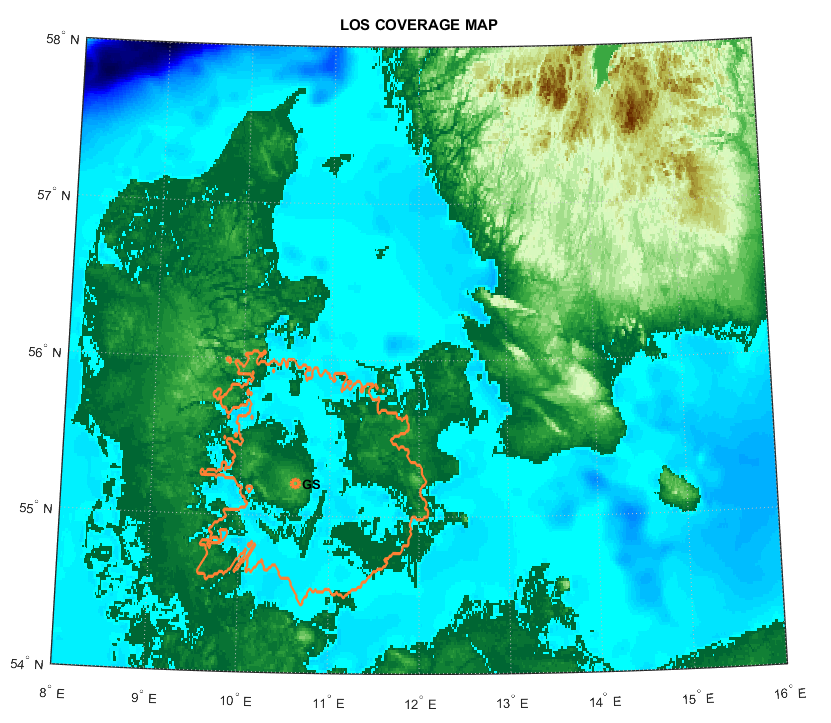
\includegraphics[scale=0.40]{../report/figures/los_odense.png}
    \end{figure}
\end{frame}

\begin{frame}{Simulation}{2D UAS}
	\begin{block}{2D UAS Block Diagram}
		\begin{itemize}
		  	\item Cartesian system (Simplistic)
		  	\item 1 DoF - azimuth angle ($\theta$)
		  	\item Compute optimal azimuth angle for UA and GS 
		\end{itemize}

		\begin{figure}
	        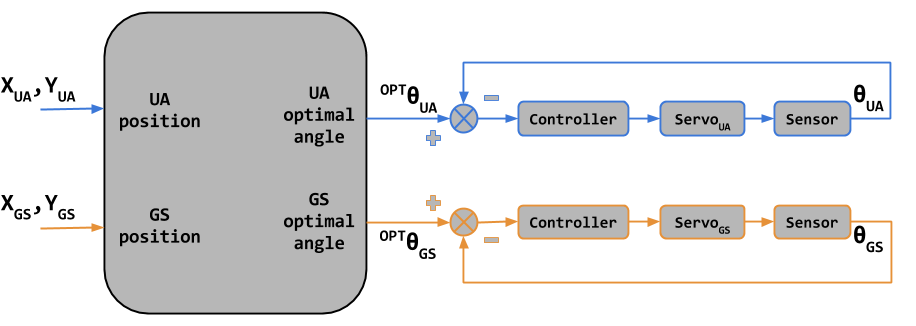
\includegraphics[scale=0.32]{figures/2D_system.png}
	    \end{figure}
    \end{block}
\end{frame}

\begin{frame}{Simulation}{3D UAS}
  \begin{block}{3D UAS Block Diagram}
	\begin{itemize}
	  	\item Realistic Earth Model - WGS84
	  	\item Curvature of the Earth
	  	\item Relief of Earth's surface 
	  	\item Real GPS position: latitude, longitude and altitude
	\end{itemize}

	\begin{figure}
		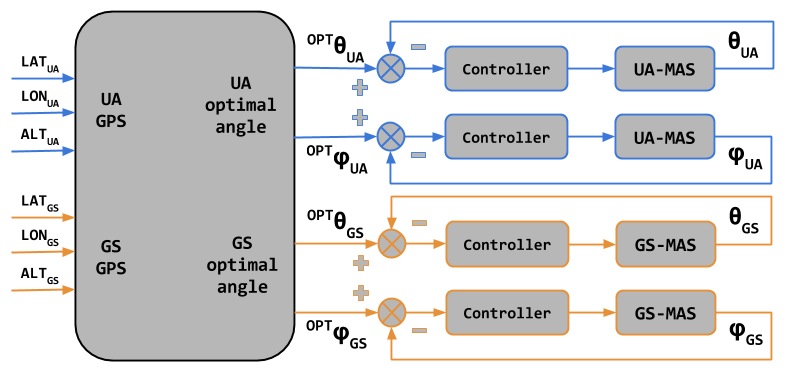
\includegraphics[scale=0.33]{figures/3D_system.png}
	\end{figure}
  \end{block}
\end{frame}

\begin{frame}{Simulation}{3D UAS}
  \begin{block}{Simulation steps}
	  \begin{enumerate}
	  	\item Aquire GPS position of GS and UA 
	  	\item Compute optimal angles and error signal 
	  	\item Input error signal in the controller
	  	\item Limit output signal from controller using the saturation box
	  	\item Input controller signal to the MAS
	  	\item Feedback the output angle in the optimal angle block
	  \end{enumerate}
  \end{block}
\end{frame}

\begin{frame}{Simulation}{3D UAS}
  \begin{block}{Simulation assumptions}
	  \begin{itemize}
	  	\item Antenna parameters for GS and UA
	  	\item Using same MAS model for GS and UA
	  	\item Controller will be defined in each simulation
	  	\item Saturation box threshold set from $-5V$ to $+5V$
	  	\item Noise modelled as Gaussian White Noise of power $10^{-4}$
	  	\item No power threshold in the receiver
	  \end{itemize}
  \end{block}
\end{frame}